\documentclass{beamer}
\usetheme{Madrid}

\usepackage[T1]{fontenc}
\usepackage{lmodern}
\usepackage{pifont}
\usepackage{comment}
\usepackage{multicol}
\usepackage{siunitx}

\usepackage{colortbl}
\usepackage{xcolor}
\usepackage{fontawesome5}
\usepackage{pifont}
\newcommand{\cmark}{\ding{51}} % ✓
\newcommand{\xmark}{\ding{55}} % ✗

\usepackage[yyyymmdd]{datetime}
\usepackage{tikz}
\usepackage{circuitikz}
\usepackage{pgfplots}

\usepackage{hyperref}
\usepackage{mathtools}
\usepackage{adjustbox}

\usepackage{animate}
%\usepackage{cite}

\usepackage[style=alphabetic,backend=biber, style=numeric, sorting=none]{biblatex}
%\addbibresource{references.bib}
\renewcommand*{\mkbibacro}[1]{#1}

\usetikzlibrary{arrows, shapes, calc, positioning}
%\usetikzlibrary{external}
%\usepgfplotslibrary{external}
%\tikzexternalize
\pgfplotsset{compat=1.18}

\renewcommand{\dateseparator}{--}

\makeatletter
\let\slideno\beamer@slideinframe
\makeatother


\DeclarePairedDelimiter\bra{\langle}{\rvert}
\DeclarePairedDelimiter\ket{\lvert}{\rangle}
\DeclarePairedDelimiterX\braket[2]{\langle}{\rangle}{#1\,\delimsize\vert\,\mathopen{}#2}

\definecolor{links}{HTML}{2A1B81}
\hypersetup{colorlinks,linkcolor=,urlcolor=links}

\definecolor{UDSgreenDurable}{RGB}{149, 193, 78}
\definecolor{UDSgreenVivacite}{RGB}{121, 181, 81}
\definecolor{UDSgreenCreativite}{RGB}{90, 173, 85}
\definecolor{UDSgreenFierte}{RGB}{0, 167, 89}
\definecolor{UDSgreenSolidarite}{RGB}{61, 143, 88}
\definecolor{UDSgreenBien-etre}{RGB}{68, 124, 90}
\definecolor{UDSgreenReussite}{RGB}{72, 106, 92} 
\definecolor{UDSgrey}{RGB}{228, 232, 225} 

\setbeamercolor{palette primary}{bg=UDSgreenSolidarite,fg=white}
\setbeamercolor{palette secondary}{bg=UDSgreenFierte,fg=white}
\setbeamercolor{palette tertiary}{bg=UDSgreenCreativite,fg=white}
\setbeamercolor{palette quaternary}{bg=UDSgreenReussite,fg=white}
\setbeamercolor{structure}{fg=UDSgreenReussite} % itemize, enumerate, etc
\setbeamercolor{section in toc}{fg=UDSgreenBien-etre} % TOC sections
\setbeamercolor{background canvas}{bg=UDSgrey}


\setbeamertemplate{caption}[numbered]


\makeatletter
\newcommand\titlegraphicii[1]{\def\inserttitlegraphicii{#1}}
\titlegraphicii{}
\setbeamertemplate{title page}
{
    {\usebeamercolor[fg]{titlegraphic}\inserttitlegraphic\hfill\inserttitlegraphicii\par}
    \begin{multicols}{2}
        \begin{beamercolorbox}[sep=8pt,center,shadow=true,rounded=true, wd=0.5\textwidth]{title}
            \usebeamerfont{title}\inserttitle\par%
            {\usebeamerfont{subtitle}\usebeamercolor[fg]{subtitle}\insertsubtitle\par}%
            {\vspace{24pt}\small\usebeamerfont{author}\insertauthor\par}%
        \end{beamercolorbox}%
    \vfill\null
    \columnbreak
    \end{multicols}
}
\makeatother
\author{Pascal-Emmanuel Lachance}
\title{PPPPP03}
\subtitle{Comment conçevoir un\\ Power Delivery Network?}
\institute{Compétitions de Conception de Circuits Imprimés}
\date{\today}
\titlegraphic{\includegraphics[scale = 0.3]{pictures/logo/udes_logo.pdf}}
%\titlegraphicii{\includegraphics[scale = 0.2]{pictures/logo/3IT_logo.png}}
%\logo{\includegraphics[scale = 0.15]{pictures/logo/udes_logo.pdf}}

\defbeamertemplate*{footline}{mytheme}
{
    \leavevmode%
    \hbox{%
    \begin{beamercolorbox}[wd=.33\paperwidth,ht=2.25ex,dp=1ex,center]{author in head/foot}%
        \usebeamerfont{author in head/foot} Pascal-Emmanuel Lachance
    \end{beamercolorbox}%
    \begin{beamercolorbox}[wd=.34\paperwidth,ht=2.25ex,dp=1ex,center]{title in head/foot}%
        \usebeamerfont{title in head/foot}\inserttitle
    \end{beamercolorbox}}%
    \begin{beamercolorbox}[wd=.33\paperwidth,ht=2.25ex,dp=1ex,right]{date in head/foot}%
        \hfill\usebeamerfont{date in head/foot}\today{}
        \hfill%\hspace*{2em}
        \insertframenumber{} / \inserttotalframenumber\hspace*{2ex} 
    \end{beamercolorbox}
}%

\defbeamertemplate*{frametitle}{mytheme}
{%
    \vspace{0cm}
    {\usebeamerfont{title}\usebeamercolor[bg]{title}\insertframetitle}
    \par
    \vspace{-0.55cm}
    \hfill
    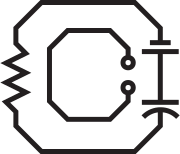
\includegraphics[height=0.635cm]{pictures/logo/c3i.png}
    \includegraphics[height=0.635cm]{pictures/logo/m1_alpha.pdf}
    \par
    \vspace{-0.3cm}
    \textcolor{UDSgreenSolidarite}{\noindent\rule{\textwidth}{1pt}}
}%

\setbeamertemplate{itemize item}{\large$\bullet$}
\setbeamertemplate{itemize subitem}{\small$\bullet$}
\setbeamertemplate{itemize subsubitem}{\tiny$\bullet$}
\usebeamertemplate{mytheme}

\newif\ifINTRO
\INTROfalse

\ifINTRO
    \includeonlyframes{intro}
    \setbeamertemplate{navigation symbols}{}
\fi



% ----------------------- BEGIN DOCUMENT ------------------------

\begin{document}

\usebackgroundtemplate{
\begin{tikzpicture}[remember picture, overlay]
        \node[at=(current page.center)] {
            {\includegraphics[height=\paperheight,keepaspectratio]{pictures/background/background-PCB.png}}
        };
    \end{tikzpicture}
}

\begin{frame}[plain]
    \maketitle
\end{frame}

\usebackgroundtemplate{
\begin{tikzpicture}[remember picture, overlay]
        \node[at=(current page.center)] {
            {\includegraphics[height=\paperheight,keepaspectratio]{pictures/background/background-pcb-poster.png}}
        };
    \end{tikzpicture}
}

\begin{frame}[plain, label=intro]
    \centering
    \Large

    \textcolor{white}{
        \LARGE{\textbf{\inserttitle}}\\
        \textbf{\textit{\insertsubtitle}}\\
        Par: \insertauthor\\
    }
    \vspace{24pt}
    \begin{tabular}{c l}
        \textcolor{UDSgreenFierte}{\faShield*}
            & \textcolor{white}{~Comment protéger une alimentation?}\\
            [0.3em]
        \textcolor{UDSgreenFierte}{\faSlidersH}
            & \textcolor{white}{~Quels sont les types de régulateurs?}\\
            [0.3em]
        \textcolor{UDSgreenFierte}{\faEquals}
            & \textcolor{white}{~À quoi sert le découplage?}\\
            [0.3em]
        \textcolor{UDSgreenFierte}{\faWaveSquare}
            & \textcolor{white}{~Comment filtrer une alimentation?}\\
            [0.3em]
        \textcolor{UDSgreenFierte}{\faProjectDiagram}
            & \textcolor{white}{~Comment conçevoir un arbre d'alimentation?}\\
    \end{tabular}
\end{frame}



% - TOC -
\usebackgroundtemplate{
\begin{tikzpicture}[remember picture, overlay]
        \node[at=(current page.center)] {
            \includegraphics[width=\paperwidth,height=\paperheight,keepaspectratio]{pictures/background/background2.jpg}
        };
    \end{tikzpicture}
}


\AtBeginSection[]{
    \begin{frame}[plain]
         \vfill
         \centering
         \begin{beamercolorbox}[sep=6pt,center,shadow=true,rounded=true]{title}
             \usebeamerfont{title}\insertsectionhead\par%
         \end{beamercolorbox}
         \tableofcontents[currentsection,hideothersubsections]
         \vfill
  \end{frame}
}

\AtBeginSubsection[]
{
    \begin{frame}[plain]
         \vfill
         \centering
         \begin{beamercolorbox}[sep=6pt,center,shadow=true,rounded=true]{title}
             \usebeamerfont{title}\insertsectionhead\par%
         \end{beamercolorbox}
         \tableofcontents[currentsection,currentsubsection,subsectionstyle=show/shaded/hide]
         \vfill
    \end{frame}
}



% ------------ SECTIONS -----------

%%!TEX root = ../main.tex 

\section{Comment protéger une alimentation?}

\subsection{Protection antistatique}

\begin{frame}{Décharge Électrostatique (ESD)}
    \begin{columns}
        \begin{column}{0.66\textwidth}
            \begin{itemize}
                \item Norme IEC-61000-4-2
                \begin{itemize}
                    \item Types de décharges
                    \item Méthodologies de tests \& certification
                    \item 4 catégories de produits
                    \item Jusqu'à $\SI{\pm 8}{\kilo\volt}$ / $\SI{\pm 15}{\kilo\volt}$
                \end{itemize}
                \item Deux types de chocs statiques
                \begin{itemize}
                    \item \textbf{Contact Discharge} - Toucher directement chaque pin avec un ESD gun
                    \item \textbf{Air Discharge} - ESD gun proche du DUT jusqu'à décharge
                \end{itemize}
            \end{itemize}
        \end{column}

        \begin{column}{0.33\textwidth}
            \begin{figure}
                \centering
                \includegraphics[width=\textwidth]{pictures/ESD-discharge-finger.png}
            \end{figure}
            \begin{figure}
                \centering
                \includegraphics[width=0.5\textwidth]{pictures/ESD-logo.png}
            \end{figure}
        \end{column}
    \end{columns}
\end{frame}

\begin{frame}{Décharge Électrostatique - Waveform}
    \begin{columns}
        \begin{column}{0.5\textwidth}
        \end{column}
        \begin{column}{0.5\textwidth}
            \begin{itemize}
                \item Pic de courant initial
                \begin{itemize}
                    \item Rise time $\lesssim \SI{1}{\nano\second}$
                \end{itemize}
                \item $2^e$ pic
                \item Chute graduelle
            \end{itemize}
        \end{column}
    \end{columns}

    \vspace{-66pt}

    \begin{figure}
        \centering
        \includegraphics[width=\textwidth]{pictures/ESD-discharge-waveform.png}
    \end{figure}
\end{frame}

\begin{frame}{Circuit protégé antistatiquement - Zener}
    \begin{center}
    \vspace{-24pt}
    \resizebox{\textwidth}{!}{
    \begin{circuitikz}[american voltages]
        \draw [thick]
        (0,-3) to [short, *-] (10,-3)
        to [european resistor, l_=${LOAD}$] (10,1)
        (0,-3) to [open, v<=$V$] (0,1)
        to [short] (10,1)
        ;

        \draw [thick]
        (3, -3) to [empty ZZener diode, color=red] (3, 1);

        % Current spike as a waveform
        \draw[thick, ->] (-0.1, 2) -- (0,3) % Rising edge
        -- (0,3) -- (0.1,1.8) % First sharp drop
        -- (0.2,2.5) -- (0.3,1.9) % Second spike
        -- (0.4,2.3) -- (0.5,2.0) % Smaller oscillation
        -- (0.6,2.15) -- (0.7,2.05) % Final damping
        -- (1,2.1); % Settling

        \node[right] at (1,2.1) {$i_{\text{ESD}}(t) \rightarrow \SI{8}{\kilo\volt}$};
    \end{circuitikz}
    }
    \end{center}
\end{frame}

\begin{frame}{Diode Normale - IV Curve}
    \begin{figure}
        \centering
        \includegraphics[width=\textwidth]{pictures/diode-iv-curve.png}
    \end{figure}
\end{frame}

\begin{frame}{Diode Zener}
    \begin{columns}
        \begin{column}{0.4\textwidth}
            \begin{itemize}
                \item \textbf{Faite pour être mise à l'envers!}
                \bigskip
                \item $V_Z$ contrôlé
                \item Beaucoup de courant en avalanche
                \item N'endommage pas la diode
                \bigskip
                \item Utilisé dans des références de tension
                \item Utilise comme protection antistatique
            \end{itemize}
        \end{column}
        \begin{column}{0.6\textwidth}
            \begin{figure}
                \centering
                \includegraphics[width=\textwidth]{pictures/diode-zener-iv-curve.png}
            \end{figure}
        \end{column}
    \end{columns}
\end{frame}

\begin{frame}{Circuit protégé antistatiquement}
    \begin{center}
    \vspace{-24pt}
    \resizebox{\textwidth}{!}{
    \begin{circuitikz}[american voltages]
        \draw [thick]
        (0,-3) to [short, *-] (10,-3)
        to [european resistor, l_=${LOAD}$] (10,1)
        (0,-3) to [open, v<=$V$] (0,1)
        to [short] (10,1)
        ;

        \draw [thick]
        (3, -3) to [full ZZener diode, a=$\SI{15}{\volt}$] (3, 1);

        \draw[->, thick, red] 
        (1, 0.75) to[out=0, in=90] (2.75, -0.5);

        % Current spike as a waveform
        \draw[thick, ->]
           (-0.1, 2) -- (0,3)       % Rising edge
        -- (0,3) -- (0.1,1.8)       % First sharp drop
        -- (0.2,2.5) -- (0.3,1.9)   % Second spike
        -- (0.4,2.3) -- (0.5,2.0)   % Smaller oscillation
        -- (0.6,2.15) -- (0.7,2.05) % Final damping
        -- (1,2.1);                 % Settling

        \node[right] at (1,2.1) {$i_{\text{ESD}}(t) \rightarrow \SI{8}{\kilo\volt}$};
    \end{circuitikz}
    }
    \end{center}
\end{frame}


\begin{frame}{Protection avec une diode Zener}
    \begin{itemize}
        \item Clamp le pulse à $V_Z$
        \item Protège les dispositifs par apprès
        \bigskip
        \item Pas l'option la plus rapide
        \item Ne protège pas contre un pulse négatif 
    \end{itemize}

    \begin{figure}
        \centering
        \includegraphics[width=\textwidth]{pictures/clamping-esd-pulse.png}
    \end{figure}
\end{frame}


\begin{frame}{Circuit protégé antistatiquement - TVS}
    \begin{center}
    \vspace{-24pt}
    \resizebox{\textwidth}{!}{
    \begin{circuitikz}[american voltages]
        \draw [thick]
        (0,-3) to [short, *-] (10,-3)
        to [european resistor, l_=${LOAD}$] (10,1)
        (0,-3) to [open, v<=$V$] (0,1)
        to [short] (10,1)
        ;

        % TODO : MODIFIER LA DIODE POUR UNE TVS

        \draw [thick]
        (3, -3) to [empty ZZener diode, color=red] (3, 1);

        % Current spike as a waveform
        \draw[thick, ->] (-0.1, 2) -- (0,3) % Rising edge
        -- (0,3) -- (0.1,1.8) % First sharp drop
        -- (0.2,2.5) -- (0.3,1.9) % Second spike
        -- (0.4,2.3) -- (0.5,2.0) % Smaller oscillation
        -- (0.6,2.15) -- (0.7,2.05) % Final damping
        -- (1,2.1); % Settling

        \node[right] at (1,2.1) {$i_{\text{ESD}}(t) \rightarrow \pm\SI{8}{\kilo\volt}$};

        \draw[->, thick, red] 
        (1, 0.75) to[out=0, in=90] (2.75, -0.5);

        \draw[->, thick, blue] 
        (1, -2.75) to[out=0, in=-90] (2.75, -1.5);
    \end{circuitikz}
    }
    \end{center}
\end{frame}

\begin{frame}{Diode TVS (Transient Voltage Suppression)}
    \begin{columns}
        \begin{column}{0.5\textwidth}
            \begin{itemize}
                \item \textbf{Faite pour protection antistatique!}
                \item \textbf{Bidirectionnel!!}
            \end{itemize}
        \end{column}
        \begin{column}{0.5\textwidth}
            \begin{itemize}
                \item Deux diodes Zener qui se font face
                \item \textit{iv curve} symmétrique
            \end{itemize}
        \end{column}
    \end{columns}
    \begin{figure}
                \centering
                \includegraphics[width=\textwidth]{pictures/diode-tvs-iv-curve.png}
            \end{figure}
\end{frame}

\begin{frame}{Circuit protégé antistatiquement - Condensateur}
    \begin{center}
    \vspace{-24pt}
    \resizebox{\textwidth}{!}{
    \begin{circuitikz}[american voltages]
        \draw [thick]
        (0,-3) to [short, *-] (10,-3)
        to [european resistor, l_=${LOAD}$] (10,1)
        (0,-3) to [open, v<=$V$] (0,1)
        to [short] (10,1)
        ;

        \draw [thick]
        (3, -3) to [C, color=red] (3, 1);

        % Current spike as a waveform
        \draw[thick, ->] (-0.1, 2) -- (0,3) % Rising edge
        -- (0,3) -- (0.1,1.8) % First sharp drop
        -- (0.2,2.5) -- (0.3,1.9) % Second spike
        -- (0.4,2.3) -- (0.5,2.0) % Smaller oscillation
        -- (0.6,2.15) -- (0.7,2.05) % Final damping
        -- (1,2.1); % Settling

        \node[right] at (1,2.1) {$i_{\text{ESD}}(t) \rightarrow \pm\SI{8}{\kilo\volt}$};
    \end{circuitikz}
    }
    \end{center}
\end{frame}


\subsection{Protection de tension inverse}
\begin{frame}{Circuit de protection inverse - Diode}
    \begin{columns}
        \begin{column}{0.33\textwidth}
            \begin{itemize}
                \item Ne conduit que dans un sens
                \bigskip
                \item Drop de tension $V_f$
                \item $P = I \cdot V_f$
            \end{itemize}
        \end{column}
        \begin{column}{0.66\textwidth}
            \begin{center}
            \vspace{-24pt}
            \resizebox{\textwidth}{!}{
            \begin{circuitikz}[american voltages]
                \draw [thick]
                (0, 0) to [short, *-] (10, 0)
                to [european resistor, l_=${LOAD}$] (10, 5)
                (0, 0) to [open, v<=$V$] (0, 5)
                to [short] (4, 5)
                to [empty diode, color=red] (6, 5)
                to [short] (10, 5)
                ;
            \end{circuitikz}
            }
            \end{center}
        \end{column}
    \end{columns}
\end{frame}

\begin{frame}{Circuit de protection inverse - Diode Schottky}
    \begin{columns}
        \begin{column}{0.33\textwidth}
            \begin{itemize}
                \item Ne conduit que dans un sens
                \bigskip
                \item Drop de tension $V_f$ plus petite
                \item $P = I \cdot V_f$
                \bigskip
                \item Plus cher pour même rating de courant
            \end{itemize}
        \end{column}
        \begin{column}{0.66\textwidth}
            \begin{center}
            \vspace{-24pt}
            \resizebox{\textwidth}{!}{
            \begin{circuitikz}[american voltages]
                \draw [thick]
                (0, 0) to [short, *-] (10, 0)
                to [european resistor, l_=${LOAD}$] (10, 5)
                (0, 0) to [open, v<=$V$] (0, 5)
                to [short] (4, 5)
                to [empty Schottky diode, color=red] (6, 5)
                to [short] (10, 5)
                ;
            \end{circuitikz}
            }
            \end{center}
        \end{column}
    \end{columns}
\end{frame}

\begin{frame}{Circuit de protection inverse - PMOS}
    \begin{columns}
        \begin{column}{0.33\textwidth}
            \begin{itemize}
                \item Ne conduit que dans un sens
                \bigskip
                \item Drop de tension vraiment plus petite ($R_{ds_{on}} \cdot I$)
                \bigskip
                \item Tension maximale supportée
            \end{itemize}
        \end{column}
        \begin{column}{0.66\textwidth}
            \begin{center}
            \vspace{-24pt}
            \resizebox{\textwidth}{!}{
            \begin{circuitikz}[american voltages]
                \draw [thick]
                (0, 0) to [short, *-] (10, 0)
                to [european resistor, l_=${LOAD}$] (10, 5)
                (0, 0) to [open, v<=$V$] (0, 5);
                
                \draw   (4,5) node[pigfete, bodydiode, color=red, rotate=90, xscale=2, yscale=-2] (fet) {}
                (fet.G) node [anchor=south, xshift=8pt] {G}
                (fet.D) node [anchor=east, yshift=8pt] {D}
                (fet.S) node [anchor=west, yshift=8pt] {S}
                (fet.G) to [short, -*] (fet.G |- 0,0)
                (fet.D) to [short, -*] (0, 5)
                (fet.S) to (10, 5);
            \end{circuitikz}
            }
            \end{center}
        \end{column}
    \end{columns}
\end{frame}

\begin{frame}{Transistor MOSFET P-Channel (PMOS)}
    \begin{columns}
        \begin{column}{0.75\textwidth}
            \begin{center}
                $V_{gs}$ négatif!\\
                \vspace{6pt}
                $V_{gs} < -V_t$
            \end{center}
            \vspace{24pt}

            \begin{columns}
                \begin{column}{0.5\textwidth}
                    \begin{itemize}
                        \item $V_G = VDD$
                        \item $V_{gs} = \SI{0}{\volt}$
                        \item $\SI{0}{\volt} > -V_t$
                        \item Ne conduit pas
                    \end{itemize}
                \end{column}
                \begin{column}{0.5\textwidth}
                    \begin{itemize}
                        \item $V_G = \SI{0}{\volt}$
                        \item $V_{gs} = -VDD$
                        \item $-VDD > -V_t$
                        \item Conduit!
                    \end{itemize}
                \end{column}
            \end{columns}
        \end{column}

        \begin{column}{0.25\textwidth}
            \begin{center}
            \vspace{-24pt}
            \resizebox{!}{0.75\textheight}{
            \begin{circuitikz}[american voltages]
                
                \draw   (2,0) node[pigfete, bodydiode, xscale=1.5, yscale=1.5] (fet) {}
                (fet.G) node [anchor=east, yshift=8pt] {G}
                (fet.D) node [anchor=south, xshift=8pt, yshift=-4pt] {D}
                (fet.S) node [anchor=north, xshift=8pt, yshift=4pt] {S}
                (fet.G) to [short, -*] (fet.G |- 0, 0.4)
                (fet.D) to [short] (2, 2)
                ++(0,0) node[vcc]{VDD}
                (fet.S) to [short] (2, -1.5)
                to [R] (2, -3.5)
                to (2, -3.75) node[ground]{}
                ;

                \draw[->, thick, red] 
                (1, 0.75) to[out=90, in=180] (1.75, 1.5);

                \node[right] at (0.66, 1.66) {$V_{gs}$};
            \end{circuitikz}
            }
            \end{center}
        \end{column}
    \end{columns}
\end{frame}

\subsection{Protection de court-circuit}
\subsection{Protection de inrush current}
\subsection{GFCI \& Grounding}
%%!TEX root = ../main.tex 

\section{Quels sont les types de régulateurs?}

\begin{frame}{Régulateurs Linéaires vs Switching}
\renewcommand{\arraystretch}{1.4}
\begin{table}
    \centering
    \begin{tabular}{>{\color{UDSgreenSolidarite}}c c | c | c}
        \rowcolor{UDSgreenSolidarite}
        \color{white}\textbf{\faList} & \color{white}\textbf{Critère} & 
        \color{white}\textbf{Régulateur Linéaire} & 
        \color{white}\textbf{Régulateur Switching} \\
        \faDollarSign\ & \textbf{Coût}       
            & {\color{UDSgreenFierte}Faible \cmark} 
            & {\color{red}Moyen à Élevé \xmark} \\
        \faPuzzlePiece\ & \textbf{Complexité} 
            & {\color{UDSgreenFierte}Faible \cmark} 
            & {\color{red}Moyen à Élevé \xmark} \\
        \faPercent\ & \textbf{Efficacité} 
            & {\color{red}Faible \xmark} 
            & {\color{UDSgreenFierte}Très Efficace \cmark} \\
        \faWaveSquare\ & \textbf{Bruit}      
            & {\color{UDSgreenFierte}Faible \cmark} 
            & {\color{red}Moyen à Élevé \xmark} \\
        \faRandom\ & \textbf{\boldmath$V_{out}$} 
            & {\color{red}$V_{out} < V_{in}$ \xmark} 
            & {\color{UDSgreenFierte}$V_{out} \subseteq \mathbb{R}$ \cmark} \\
        \faBolt\ & \textbf{Courant}            
            & {\color{red}Faible à Moyen \xmark}
            & {\color{UDSgreenFierte}Moyen à Élevé \cmark} \\
        \faThermometerHalf\ & \textbf{Température}        
            & {\color{red}Élevée \xmark}            
            & {\color{UDSgreenFierte}Faible à Moyenne \cmark} \\
    \end{tabular}
\end{table}
\end{frame}

\subsection{Régulateurs Linéaires}

\begin{frame}{Régulateur Linéaire (LDO) - Résumé}
    \begin{columns}
        \begin{column}{0.5\textwidth}
            \vspace{-24pt}
            \begin{itemize}
                \item<1-> Régulateur très simple
                \begin{itemize}
                    \item<1-> IC
                    \item<1-> Pièces autours
                \end{itemize}
                \item<2-> Output très stable
                \begin{itemize}
                    \item<2-> PSRR
                \end{itemize}
                \item<3-> $V_{in} > V_{out} > \SI{0.5}{\volt}$
                \item<4-> Très peu efficace
                \begin{itemize}
                    \setlength{\itemsep}{4pt}
                    \item<4-> $I_{in} = I_{out}$
                    \item<4-> $eff = \dfrac{P_{out}}{P_{in}} = \dfrac{V_{out}}{V_{in}}$
                \end{itemize}
                \item<5-> Power dissipée en chaleur!
                \item<5-> Limite le courant
            \end{itemize}
        \end{column}

        \begin{column}{0.5\textwidth}
            \renewcommand{\arraystretch}{1.4}
            \begin{table}
            \centering
            \begin{tabular}{>{\color{UDSgreenSolidarite}}c | c}
                \rowcolor{UDSgreenSolidarite}
                \color{white}\textbf{\faList} & \color{white}\textbf{Régulateur Linéaire}\\
                \faDollarSign\ & {\color{UDSgreenFierte}Faible \cmark}\\
                \faPuzzlePiece\ & {\color{UDSgreenFierte}Faible \cmark}\\
                \ifnum\slideno>1
                \faWaveSquare\ & {\color{UDSgreenFierte}Faible \cmark}\\
                \ifnum\slideno>2 
                \faRandom\ & {\color{red}$V_{out} < V_{in}$ \xmark}\\
                \ifnum\slideno>3 
                \faPercent\ & {\color{red}Faible \xmark}\\
                \ifnum\slideno>4 
                \faThermometerHalf\ & {\color{red}Élevée \xmark}\\
                \faBolt\ & {\color{red}Faible à Moyen \xmark}\\
                \fi\fi\fi\fi
            \end{tabular}
            \end{table}
            \vfill
            \begin{figure}
                \centering
                \includegraphics<-3>[width=0.33\textwidth]{pictures/linear-regulator-7805.png}
            \end{figure}
        \end{column}
    \end{columns}
\end{frame}

\begin{frame}{Régulateur Linéaire - Fonctionnement}
    \begin{figure}
        \centering
        \includegraphics[width=0.9\textwidth]{pictures/linear-regulator.png}
    \end{figure}
\end{frame}

\begin{frame}{Power Supply Ripple Reduction}
    \begin{columns}
        \begin{column}{0.4\textwidth}
            \begin{center}
                $PSRR = \dfrac{\Delta V_{in}}{\Delta V_{out}}$
            \end{center}
        \end{column}
        \pause
        \begin{column}{0.5\textwidth}
            \begin{center}
                $PSRR (dB) = -20 \log \left(\dfrac{\Delta V_{in}}{\Delta V_{out}}\right)$
            \end{center}
        \end{column}
    \end{columns}
    \vfill
    \begin{columns}
        \begin{column}{0.3\textwidth}
            \begin{itemize}
                \item Réduction du bruit
                \item À une fréquence
            \end{itemize}
            \pause
            \vspace{12pt}
            \begin{itemize}
                \item Graphique PSRR
                \item Dépend du courant
            \end{itemize}
        \end{column}
        \begin{column}{0.66\textwidth}
            \begin{figure}
                \centering
                \includegraphics[width=\textwidth]{pictures/psrr-graph.png}
            \end{figure}
        \end{column}
    \end{columns}
\end{frame}

\begin{frame}{Quand choisir un régulateur linéaire?}
\Large
\begin{itemize}
    \item \color{UDSgreenFierte}\faDollarSign \color{black} ~Low-Cost
    \item \color{UDSgreenFierte}\faBolt \color{black} ~Peu de courant
    \item \color{UDSgreenFierte}\faCompress \color{black} ~Peu d'espace
    \item \color{UDSgreenFierte}\faWaveSquare \color{black} ~Bruit très important
    \item \color{UDSgreenFierte}\faPercent \color{black} ~Efficacité peu importante
    \bigskip
    \item \color{UDSgreenFierte}\faLightbulb \color{black} ~À utiliser avec des régulateurs switching!
\end{itemize}

\end{frame}

\subsection{Régulateurs \textit{Switching}}
%!TEX root = ../main.tex 

\section{Comment une impédance?}

\subsection{Matching à la source}

\begin{frame}{Matching à la source}
    \begin{itemize}
        \item Plupart des circuits avec sortie CMOS
        \item $Z_o \rightarrow 0\Omega$
    \end{itemize}
    \begin{columns}
        \begin{column}{0.25\textwidth}
            \begin{center}
                \begin{figure}
                \centering
                \includegraphics[width=\textwidth]{pictures/CMOS_inverter.png}
            \end{figure}
            \end{center}
        \end{column}
        \begin{column}{0.75\textwidth}
            \begin{center}
                \resizebox{\textwidth}{!}{
                \ctikzset{bipoles/resistor/height=0.1}
                \ctikzset{bipoles/resistor/width=0.3}
                \begin{circuitikz}[american voltages]
                    \draw [thick]
                    (0,0) to [short, *-] (10,0)
                    to [european resistor, l=$Z_L$] (10, 4)
                    (0,0) to [open, v<=$V_S$] (0,4)
                    to [short, *-] (1, 4)
                    to [amp, a=$Z_o \rightarrow 0$] (3, 4)
                    to [short] (6, 4)
                    to [european resistor, l=$Z_0$] (8, 4)
                    to [short] (10,4)
                    ;
                    \draw
                    (0, 0) to [open] (1.25, 4)
                    to [R] (2.75, 4)
                    ;
                \end{circuitikz}
                }
            \end{center}
        \end{column}
    \end{columns}
\end{frame}

\begin{frame}{Matching à la source - Résistance série}
    \begin{columns}
        \begin{column}{0.3\textwidth}
            \begin{itemize}
                \item Ajouter une résistance externe!
                \item Très proche de la sortie
                \bigskip
                \item Valider $Z_o$ du IC
                \item $Z_S = Z_0 - Z_o$
            \end{itemize}
        \end{column}
        \begin{column}{0.7\textwidth}
            \begin{center}
            \resizebox{\textwidth}{!}{
            \ctikzset{bipoles/resistor/height=0.1}
            \ctikzset{bipoles/resistor/width=0.3}
            \begin{circuitikz}[american voltages]
                \draw [thick]
                (0,0) to [short, *-] (10,0)
                to [european resistor, l=$Z_L$] (10, 4)
                (0,0) to [open, v<=$V_S$] (0,4)
                to [short, *-] (1, 4)
                to [amp, a=$Z_o \rightarrow 0$] (3, 4)
                to [european resistor, l=$Z_S$, color=red] (5, 4)
                to [short] (6, 4)
                to [european resistor, l=$Z_0$] (8, 4)
                to [short] (10,4)
                ;
                \draw
                (0, 0) to [open] (1.25, 4)
                to [R] (2.75, 4)
                ;
            \end{circuitikz}
            }
            \end{center}
        \end{column}
    \end{columns}
\end{frame}


\subsection{Matching à la load}

\begin{frame}{Matching à la load}
    \begin{itemize}
        \item Plupart des circuits avec entrée CMOS
        \item $Z_L \rightarrow \infty\Omega$
    \end{itemize}
    \begin{columns}
        \begin{column}{0.25\textwidth}
            \begin{center}
                \begin{figure}
                \centering
                \includegraphics[width=\textwidth]{pictures/CMOS_inverter.png}
            \end{figure}
            \end{center}
        \end{column}
        \begin{column}{0.75\textwidth}
            \begin{center}
                \resizebox{\textwidth}{!}{
                \ctikzset{bipoles/resistor/height=0.1}
                \ctikzset{bipoles/resistor/width=0.3}
                \begin{circuitikz}[american voltages]
                    \draw [thick]
                    (0,0) to [short, *-] (10,0)
                    to [open] (10, 4)
                    (0,0) to [open, v<=$V_S$] (0,4)
                    to [short, *-] (1, 4)
                    to [amp, a=$Z_o \rightarrow 0$] (3, 4)
                    to [european resistor, l=$Z_S$] (4.25, 4)
                    to [european resistor, l=$Z_0$] (7, 4)
                    to [amp, a=$Z_i \rightarrow \infty$] (10, 4)
                    ;
                    \draw
                    (0, 0) to [open] (1.25, 4)
                    to [R] (2.75, 4)
                    ;
                \end{circuitikz}
                }
            \end{center}
        \end{column}
    \end{columns}
\end{frame}

\begin{frame}{Matching à la load - Résistance parallèle}
    \begin{columns}
        \begin{column}{0.3\textwidth}
            \begin{itemize}
                \item Ajouter une résistance externe!
                \item Très proche de l'entrée
                \bigskip
                \item Valider $Z_i$ du IC
                \item $Z_L = Z_0 - \frac{Z_0}{Z_i}$
            \end{itemize}
        \end{column}
        \begin{column}{0.7\textwidth}
            \begin{center}
            \resizebox{\textwidth}{!}{
            \ctikzset{bipoles/resistor/height=0.1}
            \ctikzset{bipoles/resistor/width=0.3}
            \begin{circuitikz}[american voltages]
                \draw [thick]
                    (0,0) to [short, *-] (10,0)
                    to [open] (10, 4)
                    (0,0) to [open, v<=$V_S$] (0,4)
                    to [short, *-] (1, 4)
                    to [amp, a=$Z_o \rightarrow 0$] (3, 4)
                    to [european resistor, l=$Z_S$] (4.25, 4)
                    to [european resistor, l=$Z_0$] (7, 4)
                    to [amp, a=$Z_i \rightarrow \infty$] (10, 4)
                    ;
                \draw [thick]
                    (7.5, 4) to [european resistor, l=$Z_L$, color=red] (7.5, 0)
                    ;
                \draw
                    (0, 0) to [open] (1.25, 4)
                    to [R] (2.75, 4)
                    ;

            \end{circuitikz}
            }
            \end{center}
        \end{column}
    \end{columns}
\end{frame}

\subsection{Matching du conducteur}

\begin{frame}{Impédance caractéristique}
    \begin{itemize}
        \item L'impédance caractéristique $Z_0$ d'une ligne de transmission
        \item Ne dépend que de la \textit{géométrie} de la ligne de transmission
        \item Contrôle les éléments capacitifs et inductifs parasites, qui dominent
        \bigskip
        \item Augmenter largeur de trace $\rightarrow$ plus de capacitance
        \item Augmenter distance entre les traces $\rightarrow$ plus d'inductance
        \bigskip
        \item \textit{Dans un PCB, l'inductance parasite domine toujours!}
    \end{itemize}
\end{frame}

\begin{frame}{Géométries}
    \begin{center}
        \begin{figure}
            \centering
            \includegraphics[width=\textwidth]{pictures/microstrip-VS-Stripline-vs-coplanar-waveguide.png}
        \end{figure}
    \end{center}
\end{frame}

\begin{frame}{Microstrip}
    \begin{columns}
        \begin{column}{0.66\textwidth}
            \begin{itemize}
                \item Trace sur le TOP / BOTTOM du PCB
                \item Plan de retour en-dessous de la trace
                \item Diélectrique d'un seul côté
                \item Signal plus rapide
            \end{itemize}
        \end{column}
        \begin{column}{0.33\textwidth}
            \begin{center}
                \begin{figure}
                    \centering
                    \includegraphics[width=\textwidth]{pictures/microstrip.png}
                \end{figure}
            \end{center}
        \end{column}
    \end{columns}
\end{frame}

\begin{frame}{Microstrip - Formule}
    \begin{itemize}
        \item Norme IPC-2141
        \item Approximation empirique
    \end{itemize}
    \pause
    \begin{center}
        \[
            Z_0 =
            \begin{cases} 
                \dfrac{60}{\sqrt{\varepsilon_{eff}}}\ln\left(8\frac{H}{W} + 0.25\frac{W}{H}\right), & \text{if } \frac{W}{H} < 1 \\
                \dfrac{120 \pi}{\sqrt{\varepsilon_{eff}} \cdot \left(\frac{W}{H} + 1.393 + \frac{2}{3}\ln\left(\frac{w}{H} + 1.444\right)\right)}, & \text{if } \frac{W}{H} \geq 1
            \end{cases}
        \]
        \[
            \varepsilon_{eff} \coloneqq
            \begin{cases} 
                \frac{\varepsilon_r + 1}{2} + \frac{\varepsilon_r - 1}{2} \cdot \left(\left(1 + 12 \frac{H}{W}\right)^{-\frac{1}{2}} + 0.04\left(1 - \frac{W}{H}\right)^2\right), & \text{if } \frac{W}{H} < 1 \\
                \frac{\varepsilon_r + 1}{2} + \frac{\varepsilon_r - 1}{2} \cdot \left(1 + 12 \frac{H}{W}\right)^{-\frac{1}{2}}, & \text{if } \frac{W}{H} \geq 1
            \end{cases}
        \]
    \end{center}
\end{frame}

\subsection{Impédance Différentielle}
%%!TEX root = ../main.tex 

\section{Comment conçevoir un arbre d'alimentation?}

\subsection{Bilan d'alimentation}
\subsection{Efficacité}
\subsection{Séquençage}



% - END -

\usebackgroundtemplate{
\begin{tikzpicture}[remember picture, overlay]
        \node[at=(current page.center)] {
            {\includegraphics[height=\paperheight,keepaspectratio]{pictures/background/background-PCB.png}}
        };
    \end{tikzpicture}
}
\begin{frame}
    \begin{multicols}{2}
        \begin{beamercolorbox}[sep=8pt,center,shadow=true,rounded=true, wd=0.5\textwidth]{title}
            {\usebeamerfont{title}Merci!\par}%
        \end{beamercolorbox}%
    \vfill\null
    \columnbreak
    \end{multicols}
\end{frame}


\end{document}
